\documentclass[10pt]{article}

% Packages
\usepackage[left=1.75cm,right=1.75cm,top=2cm,bottom=2cm]{geometry}
\usepackage{amsmath, amssymb}
\usepackage{graphicx}
\usepackage{csvsimple}
\usepackage{caption}
\usepackage{subcaption}
\usepackage{enumitem}
\usepackage{hyperref}
\usepackage{fancyhdr}
\usepackage{titlesec}
\usepackage{etoolbox}
\usepackage{makecell} % For multi-line headers#
\usepackage{adjustbox}
\usepackage[table]{xcolor}
\usepackage{array}
\usepackage{booktabs}
\usepackage{siunitx}
\usepackage{ragged2e}
\usepackage{blindtext}
\usepackage[nameinlink]{cleveref}


% Header/Footer
\pagestyle{fancy}
\fancyhf{}
\rhead{ML Project Report: Fake News Detection}
\lhead{Philipp Hoffmann, Martin Wagner}
\cfoot{\thepage}

% Section formatting
\titleformat{\section}{\large\bfseries}{\thesection}{1em}{}
\titleformat{\subsection}{\normalsize\bfseries}{\thesubsection}{1em}{}

% Title
\title{\textbf{Machine Learning Project Report: Fake News Detection}}
\author{Philipp Hoffmann, Martin Wagner \\
	Applied ML – Ludwig-Maximilians-Universität München \\
	\texttt{\href{mailto:philipp.hoffmann@campus.lmu.de}{philipp.hoffmann@campus.lmu.de}},
	\texttt{\href{mailto:wagner.mar@campus.lmu.de}{wagner.mar@campus.lmu.de}}}
\date{\today}





\begin{document}
	
	\maketitle
	\section{Task Overview}
	Due to the enormous amount of news published every day, distinguishing between fake and real news is becoming an increasingly difficult task for humans, making the use of computer models indispensable. In this project, we tested different models and text preprocessing methods using the "fake-and-real-news-dataset"\footnote{\url{https://www.kaggle.com/datasets/clmentbisaillon/fake-and-real-news-dataset}}. This dataset collects titles and texts of more than 40000 news articles classified as fake or true news.
	
	\section{Methods}
	We compared the performance of logistic regression and linear SVM models (mainly on the collection of titles) using different vectorization techniques from natural language processing. 
	We used \texttt{TfidfVectorizer} and \texttt{CountVectorizer} from \texttt{scikit-learn} for basic text vectorization, which also handle tokenization, including lower-casing and punctuation removal.\\
	Given a vocabulary of tokens (e.g. words), bag-of-words assigns to a document $d$ for each token $t$, the term-frequency $\operatorname{tf}(t,d)$, defined as the count of term $t$ in $d$ divided by the total number of terms.\footnote{Usually bag-of-words is defined without dividing by the total number of terms, but this does not matter for us, as we normalize anyway}
	 A bit more evolved is TF-IDF vectorization, which also takes into account the frequency of how often a term occurs in a fixed corpus $D=\{d_1, \dots, d_n\}$ of documents $d_1, \dots, d_n$. Given a term $t$, the inverse-document frequency of $t$ in $D$ is $\operatorname{idf}(t,D):=1+\log\left(\frac{1+n}{1+\operatorname{df}(t)}\right)$, where $\operatorname{df}(t)$ is the number of documents in $D$ containing the term $D$.\footnote{Often times one also defines  $\operatorname{idf}(t,D):=\log\left(\frac{n}{1+\operatorname{df}(t)}\right)$, but we stick with the convention implemented in \texttt{scikit-learn}} Then the TF-IDF-score of a term $t$ with respect to the collection $D$ is defined as \[\operatorname{TF-IDF}(t,d,D):=\operatorname{tf}(t,d)\operatorname{idf}(t,D).\]
	Note that $d$ does not need to be contained in the collection $D$ of documents itself. We applied $L2$-normalization to the obtained vectors and additionally applied Z-score normalization to the resulting feature matrices, as this yielded better results, particularly for linear SVM. 
	We adopted models in \texttt{courselib} to support sparse matrix operations and implemented methods to adapt to feature shifts (due to Z-score normalization) without destroying the computational efficiency resulting from the sparsity of the unshifted feature matrices. Moreover, we implemented custom tokenizers using \texttt{nltk} that support stemming and lemmatization, i.e. reduce words to a more basic form. To test all these options more compactly, we implemented a multi-column vectorizer that supports vectorization of text data from one or multiple columns of a dataframe with various vectorization options.

	
	\section{Experiments and Results}
	As both bag-of-words and TF-IDF yield highly sparse, high-dimensional vectors, one expects the problem to be linearly separable, thus we restricted our experiments to linear models, namely logistic regression and linear SVM. For all our experiments, we used an 80/20 train-test split. We labeled true news with $1$ and fake news with $0$ (for logistic regression) or $-1$ (for linear SVM), respectively. All of our models were trained for a total of 100 epochs. \\
	\indent
	We compared the models on TF-IDF vectorized text data with good-performing learning rates with full batch size. While both models achieved almost perfect train accuracy, logistic regression performed slightly better and faster. Smaller batch sizes could not improve results, but slowed down the training time significantly (see \Cref{Fig 1}). Because of this, we only used the logistic regression model with full batch size for further experimentation. 
	
	


\begin{figure}[htbp]
	\centering
	
	% First row: Two images side-by-side
	\begin{subfigure}[t]{0.48\textwidth}
		\centering
		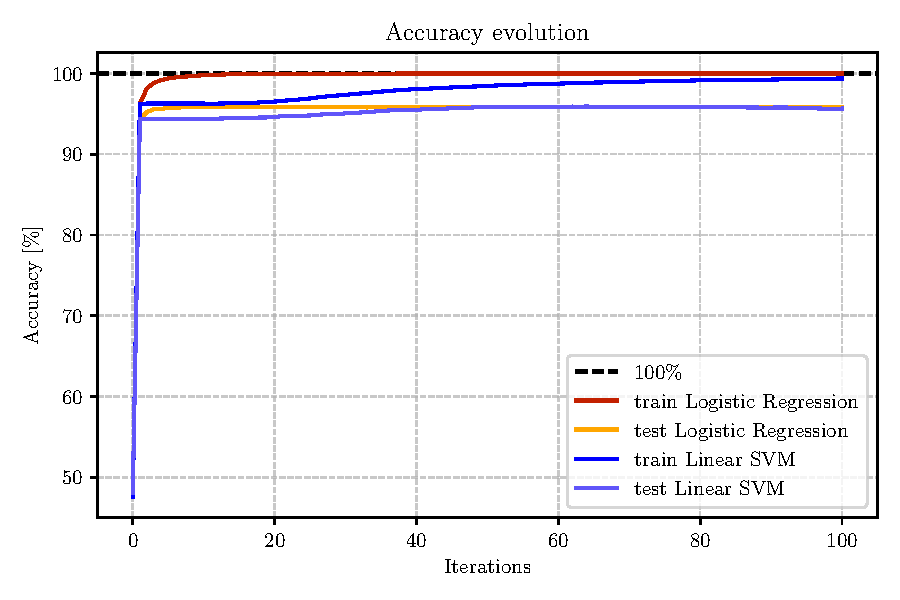
\includegraphics[height=5.2cm]{figures/model_comparison_accuracy_evolution.pdf}
		\caption{}
		\label{fig:accuracy}
	\end{subfigure}
	\hfill
	\begin{subfigure}[t]{0.48\textwidth}
		\centering
		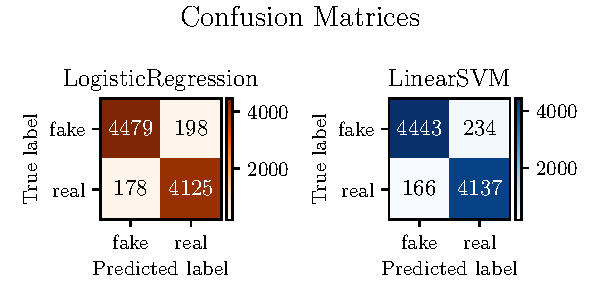
\includegraphics[height=4cm]{figures/model_comparison_confusion_matrices.pdf}
		\caption{}
		\label{fig:confusion}
	\end{subfigure}
	
	\vspace{1em} % Vertical spacing between images and table
	
	% Second row: Centered table
	\begin{subfigure}[t]{\textwidth}
		\centering
		\small
		\setlength{\tabcolsep}{4pt}
		\renewcommand{\arraystretch}{1.1}
		\begin{adjustbox}{scale=.8, center}
			\rowcolors{2}{lightgray}{white}
			\begin{tabular}{|l|c|c|c|r|r|r|r|r|r|}
				\hline
				\rowcolor{gray!30}
				\textbf{Model} & \textbf{batch size} & \textbf{learning rate} & \textbf{C} &
				 \textbf{\makecell{Train\\Accuracy\\{\footnotesize[\%]}}} & 
				\textbf{\makecell{Test\\Accuracy\\{\footnotesize[\%]}}} & 
				\textbf{\makecell{Training\\Time\\{\footnotesize[s]}}} & 
				\textbf{Precision} & \textbf{Recall} & \textbf{F1-Score} \\
				\hline
				\csvreader[
				late after line=\\\hline
				]{tables/model_comparison_table.csv}{}%
				{\csvcoli & \csvcolii & \csvcoliii & \csvcoliv & \csvcolv & \csvcolvi & \csvcolvii & \csvcolviii & \csvcolix & \csvcolix}%
			\end{tabular}
		\end{adjustbox}
		\caption{}

	\end{subfigure}
	
	\caption{Model comparison between logistic regression and linear SVM. (a): Accuracy evolution on full batch, (b): Corresponding confusion matrices, (c): Comparison of mini batch and full batch}
	\label{Fig 1}
\end{figure}

	For the second part of our experiment, we tested different vectorization methods. \Cref{Fig 2}(a) shows how the number of features affects the accuracy: In general, more features result in better accuracy, but more than 5000 features yield only a minor improvement. This trend is also confirmed by \Cref{Fig 2}(b): When using text or text and titles as data, the number of features increases significantly, while also resulting in even better test accuracy.\\
	\begin{figure}[htbp]
		\centering
		\begin{minipage}[t]{0.35\textwidth}
			\centering
			\vspace{0pt} % Reset top alignment reference
			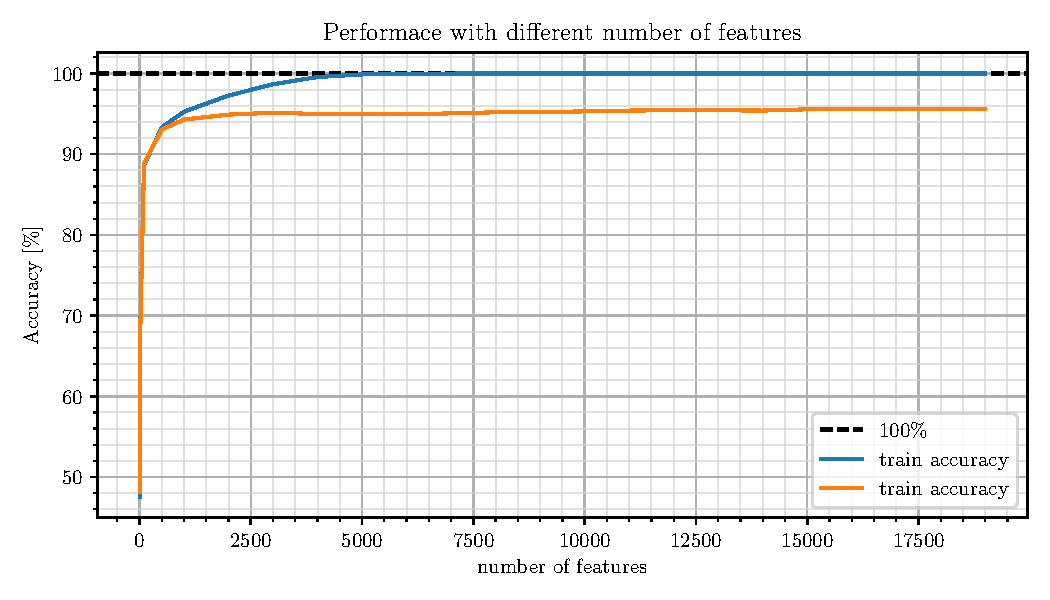
\includegraphics[height=5.3cm]{figures/vectorization_comparison_feature_number_impact.pdf}
			\subcaption{}
	
		\end{minipage}
		\hfill
		\begin{minipage}[t]{0.6\textwidth}
			\vspace{5pt} % Reset top alignment reference
			
			% First table (b)
			\small
			\setlength{\tabcolsep}{4pt}
			\renewcommand{\arraystretch}{1.1}
			\begin{adjustbox}{scale=.8, valign=t}
				\rowcolors{2}{lightgray}{white}
				\begin{tabular}{|l|c|r|r|r|r|r|}
					\hline
					\rowcolor{gray!30}
					\bfseries Data & 
					\bfseries{learning rate} &
					\bfseries Features & 
					\bfseries \makecell{Train\\Accuracy\\{\footnotesize[\%]}} & 
					\bfseries \makecell{Test\\Accuracy\\{\footnotesize[\%]}} & 
					\bfseries \makecell{Vectorization\\Time\\{\footnotesize[s]}} & 
					\bfseries \makecell{Training\\Time\\{\footnotesize[s]}} \\
					\hline
					\csvreader[
					late after line=\\\hline
					]{tables/vectorization_more_text_data.csv}{}%
					{\csvcoli  & \csvcolii & \csvcoliii & \csvcoliv & \csvcolv & \csvcolvi & \csvcolvii}%
				\end{tabular}
			\end{adjustbox}
			\subcaption{}

			
			\vspace{10pt} % Reduced vertical spacing
			
			% Second table (c)
			\small
			\setlength{\tabcolsep}{4pt}
			\renewcommand{\arraystretch}{1.1}
			\begin{adjustbox}{scale=.8, valign=t}
				\rowcolors{2}{lightgray}{white}
				\begin{tabular}{|c|c|r|r|r|r|r|}
					\hline
					\rowcolor{gray!30}
					\bfseries \makecell{n-gram\\range} & 
					\bfseries{learning rate} &
					\bfseries Features & 
					\bfseries \makecell{Train\\Accuracy\\{\footnotesize[\%]}} & 
					\bfseries \makecell{Test\\Accuracy\\{\footnotesize[\%]}} & 
					\bfseries \makecell{Vectorization\\Time\\{\footnotesize[s]}} & 
					\bfseries \makecell{Training\\Time\\{\footnotesize[s]}} \\
					\hline
					\csvreader[
					late after line=\\\hline
					]{tables/comparison_ngrams.csv}{}%
					{\csvcoli & \csvcolii & \csvcoliii & \csvcoliv & \csvcolv & \csvcolvi & \csvcolvii}%
				\end{tabular}
			\end{adjustbox}
			\subcaption{}
		\end{minipage}
		
		\caption{(a): Impact of number of features, (b): Performance with different data, (c): Influence of n-gram ranges, n-gram range given as minimum length - maximum length}
		\label{Fig 2}
	\end{figure}
	

	
		
	With that in mind, we compared TF-IDF as well as bag-of-words vectorization using four different tokenization methods, with and without stop word removal. As \Cref{table 1} highlights, all combinations achieved similar performance, but stop word removal slightly decreases test accuracy. Moreover, our custom tokenizers improved the test accuracy slightly, but the vectorization time increased heavily with the complexity of the tokenizer. \newline\newline
	
	\begin{table}[h!]
		\centering
		\small
		\setlength{\tabcolsep}{4pt}
		\renewcommand{\arraystretch}{1.1} % Increase row height for better spacing
		
		\label{tab:results}
		\begin{adjustbox}{scale=.8}
			\rowcolors{2}{lightgray}{white} % Alternate row colors
			\begin{tabular}{|l|l|l|r|r|r|r|r|r|r|}
				\hline
				\rowcolor{gray!30} % Header background color
				\bfseries Vectorization & \bfseries Stop Words & \bfseries Tokenizer & \bfseries Features & 
				\bfseries \makecell{Train\\Accuracy\\{\footnotesize[\%]}} & 
				\bfseries \makecell{Test\\Accuracy\\{\footnotesize[\%]}} & 
				\bfseries Precision & \bfseries Recall & \bfseries F1-Score & 
				\bfseries \makecell{Vectorization\\Time\\{\footnotesize[s]}} \\
				\hline
				\csvreader[
				late after line=\\\hline
				]{tables/vectorization_comparison_table.csv}{}%
				{\csvcoli & \csvcolii & \csvcoliii & \csvcoliv & \csvcolv & \csvcolvi & \csvcolvii & \csvcolviii & \csvcolix & \csvcolx}%
			\end{tabular}
			
		\end{adjustbox}
		
		\vspace{0.2cm}
		
		\caption{Comparison of different vectorization configurations with four different tokenizers. default: default tokenization from \texttt{TfIdfVectorizer}/\texttt{CountVectorizer} without custom tokenizer, basic: \texttt{nltk.word\_tokenize} combined with punctuation removal and lowercasing, stemming: basic tokenizer combined with \texttt{SnowballStemmer} from \texttt{nltk}, lemmatization: basic tokenizer combined with \texttt{WordNetLemmatizer} from \texttt{nltk}. (used learning rate: 10)}
		\label{table 1}
	\end{table}
	
	
	Lastly, we investigated which words or short phrases the model identified as most relevant for distinguishing between real and fake news (\Cref{Fig 3}). For this, we trained the model on different combinations of n-grams. \Cref{Fig 2}(c) shows that training only with bi- and especially trigrams significantly decreased the test accuracy.







	\begin{figure}[h!]
		\centering
		\includegraphics[width=.85\textwidth]{figures/wordclouds.pdf}
		\caption{Illustration of the most important n-grams identified by the model trained only on uni-, bi-, trigrams resp.}
		\label{Fig 3}
	\end{figure}
	

	
	
	\section{Discussion}
	Our experiment shows that linear models are indeed well-suited for detecting fake news, even when analyzing only news titles. If one also trains the model on the whole body of text, almost perfect classification is achievable. Removing stop words from the titles seems to worsen the performance, which could indicate that titles become too short or that they are indeed more common in either fake or real news. It seems like machine learning models prefer single words for classification, whereas humans usually need context for understanding text. However, our models only give binary classification and cannot detect the exact passages containing fake news, which could be an interesting objective for future research. A starting idea for this could be to divide the text into smaller paragraphs. 
	
	
\end{document}